\chapter{La recommendation}

\section{Introduzione}

Come fa \textit{Spotify} a sapere quale canzone l'utente vorrebbe ascoltare? E come fa \textit{Netflix} a suggerire la prossima serie da guardare? Questo è possibile grazie al modello di \textit{recommendation} basato su \textit{machine learning} che analizza cosa piace all'utente e gli propone contenuti su misura. Di solito si utilizzano due tipi principali di raccomandazioni:

\begin{itemize}
    \item per la \textit{home page}: sono raccomandazioni personalizzati per un utente in base ai suoi interessi. Ogni utente vede articoli diversi
    \item su articoli correlati: sono raccomandazioni simili a un articolo specifico. Per esempio in \textit{Google Play}, gli utenti che visualizzano la pagina di un'app di matematica potrebbero vedere anche un riquadro con app correlate, come altre app di matematica o di scienze
\end{itemize}

Un sistema di \textit{recommendation} aiuta gli utenti a scoprire contenuti interessanti all'interno di un'enorme quantità di dati. Per esempio su \textit{YouTube} ci sono miliardi di video, con nuovi contenuti che vengono aggiunti ogni giorno. Come può un utente trovare qualcosa di nuovo che valga la pena guardare o provare? La ricerca manuale è un'opzione. Tuttavia, un motore di raccomandazione è in grado di suggerire contenuti che magari l'utente non avrebbe mai pensato di cercare da solo. Basti sapere che, secondo quanto dice la pagina di \href{https://developers.google.com/machine-learning/recommendation/overview}{Google Developers - Recommendation Systems Overview}:

\begin{itemize}
    \item il 40\% delle app installate dal \textit{Google Play} derivano da raccomandazioni
    \item il 60\% del tempo di visualizzazione su \textit{YouTube} proviene dalle raccomandazioni
\end{itemize}


\subsubsection{Terminologia}
Ci sono alcuni termini da introdurre:

\begin{itemize}
    \item \textit{item}: sono gli elementi/entità raccomandate dal sistema. Su \textit{Spotify} sono le canzoni, su \textit{Amazon} sono i prodotti, su \textit{Intragram} sono i \textit{post}
    \item \textit{query}: sono le informazioni utilizzate da un sistema per fornire raccomandazioni. Le \textit{query} possono essere una combinazione di informazioni dell'utente (e.g. ID, elementi con i quali ha interagito in passato etc.) e contesto aggiuntivo (e.g. ora del giorno, per quanto tempo ha osservato quel prodotto o quell'episodio etc.)
\end{itemize}

I passaggi tipici che ti utilizzano sono: 

\begin{enumerate}
    \item generazione dei candidati: il sistema parte da un corpus di \textit{item}, potenzialmente enorme, e ne estrae un sottoinsieme molto più piccolo di candidati
    \item calcolo dello \textit{score}: un altro modello, più preciso del primo dato che lavora su una quantità molto minore di dati, assegna un punteggio ai candidati
    \item \textit{re-ranking}: i candidati vengono ordinati per lo score ricevuto considerando eventuali ulteriori vincoli (e.g. rimuovendo contenuti che l'utente ha segnalato come non graditi, oppure aumentare il punteggio di contenuti più recenti). Il riordinamento può garantire maggiore varietà, attualità e imparzialità
\end{enumerate}

\section{Generazione dei candidati}\label{generazione_dei_candidati}

La descrizione che segue riguarda soprattutto i metodi più moderni: alcuni algoritmi come \textit{KNN}~\ref{knn} o \textit{SlopeOne}~\ref{slopeone} utilizzano metodi più semplici ma comunque efficaci per il calcolo delle raccomandazioni.

\subsection{Recommendation Tasks}

Numerosi compiti di raccomandazione sono stati studiati negli ultimi decenni. Alcuni esempi di applicazioni:

\begin{itemize}
    \item raccomandazioni di film
    \item raccomandazioni di notizie
    \item raccomandazioni di punti di interesse (\textit{Point-of-Interest}~\cite{Ye})
    \item etc
\end{itemize}

È anche possibile classificare i compiti in base al tipo di feedback e ai dati in input. Alcuni esempi:

\begin{itemize}
    \item predizione del \textit{rating}: predizione delle valutazioni esplicite fornite dagli utenti    
    \item \textit{top-N recommendation} (\textit{ranking}): ordinamento personalizzato di tutti gli oggetti per ciascun utente, basato su feedback implicito    
    \item \textit{sequence-aware recommendation}: se sono disponibili informazioni temporali (\textit{timestamp}), è possibile costruire raccomandazioni che tengano conto dell’ordine delle interazioni~\cite{Quadrana}.
    \item \textit{click-through rate prediction} (\textit{CTR}): previsione della probabilità che un utente clicchi su un oggetto, utilizzando feedback implicito e molte caratteristiche categoriali
    \item \textit{cold-start recommendation}: raccomandazioni in scenari con nuovi utenti o nuovi oggetti, per cui mancano dati storici sufficienti~\cite{Schein}
\end{itemize}

\subsection{Embedding}
Gli \textit{item} e le \textit{query} vengono mappati su  vettore di \textit{embedding} in uno spazio comune $E = \mathbb{R}^k$. Normalmente lo spazio di \textit{embedding} ha una dimensione molto più piccola rispetto alla grandezza del corpus e cattura alcune strutture latenti dell'insieme di \textit{item} o \textit{query}. Gli elementi tra loro simili finiscono per essere vicini nello spazio di \textit{embedding}. Il concetto di ``vicinanza" è definito da una misura di similarità.
 
\subsection{Calcolo della similarità}

Una misura di similarità è una funzione $s: E \times E \to \mathbb{R}$ che prende in input una coppia di vettori di \textit{embedding} e restituisce un valore scalare che ne misura la similarità. Gli \textit{embedding} possono essere utilizzati per la generazione dei candidati come segue: dato un vettore di \textit{embedding} per una query $q \in E$, il sistema cerca gli \textit{embedding} degli elementi $x \in E$ che sono vicini a $q$, ossia, gli \textit{embedding} con una similarità elevata.

Per determinare il grado di similarità, la maggior parte dei sistemi di \textit{recommendation} si basa su una o più delle seguenti misure:

\begin{itemize}
    \item coseno: semplicemente il coseno dell'angolo tra i due vettori $s(q, x) = cos(q, x)$
    \item prodotto scalare: è dato da: $s(q, x) = \langle q, x \rangle = \sum\limits_{i=1}^{d} q_i x_i$. È anche dato da $s(q, x) = \|x\| \|q\| \cos(q, x)$ che corrisponde al coseno dell'angolo moltiplicato per il prodotto delle norme. Pertanto, se gli \textit{embedding} sono normalizzati, il prodotto scalare e il coseno coincidono    
    \item distanza euclidea: questa è la distanza usuale nello spazio euclideo $s(q, x) = \|q - x\| = \left[ \sum\limits_{i=1}^{d} (q_i - x_i)^2 \right]^{\frac{1}{2}}$. Una distanza minore indica una similarità maggiore. Da notare che, quando gli \textit{embedding} sono normalizzati, la distanza euclidea al quadrato coincide con il prodotto scalare (e il coseno) fino a una costante, poiché in quel caso $\frac{1}{2} \|q - x\|^2 = 1 - \langle q, x \rangle$
\end{itemize}


\begin{figure}[H]
    \centering
    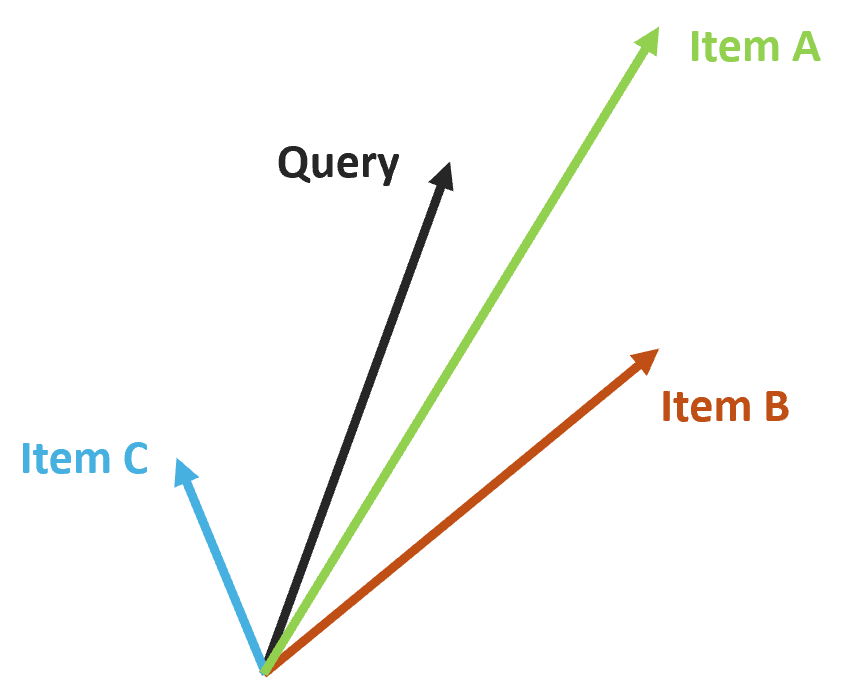
\includegraphics[scale=0.8]{figures/embedding.PNG}
    \caption{Il vettore nero illustra l'\textit{embedding} della \textit{query}. Gli altri tre vettori di \textit{embedding} (\textit{Item A}, \textit{Item B}, \textit{Item C}) rappresentano gli \textit{item} candidati. A seconda della misura di similarità utilizzata, la classifica degli elementi può essere diversa}
    \label{fig:embedding}
\end{figure}

Rispetto al coseno, la similarità del prodotto scalare è sensibile alla norma dell'\textit{embedding}. Cioè, maggiore è la norma di un \textit{embedding}, maggiore sarà la similarità e più è probabile che l'\textit{item} venga raccomandato. Questo può influenzare le raccomandazioni nei seguenti modi:

\begin{itemize}
    \item gli elementi che appaiono molto frequentemente nel \textit{training set} (ad esempio, le top canzoni italiane del momento su \textit{Spotify}) tendono ad avere \textit{embedding} con norme grandi. Se è desiderabile catturare informazioni sulla popolarità, allora si dovrebbe preferire il prodotto scalare. Tuttavia, se non si presta attenzione, gli elementi popolari potrebbero finire per dominare le raccomandazioni. In pratica, si possono utilizzare altre varianti delle misure di similarità che pongono meno enfasi sulla norma dell'\textit{item}. Ad esempio, definire $s(q, x) = \|q\|^{\alpha} \|x\|^{\alpha} \cos(q, x)$ per qualche $\alpha \in (0,1)$
    \item Gli elementi che appaiono molto raramente potrebbero non essere aggiornati frequentemente durante l'addestramento. Di conseguenza, se vengono inizializzati con una norma elevata, il sistema potrebbe raccomandare elementi rari invece di quelli più rilevanti. Per evitare questo problema, prestare attenzione all'inizializzazione degli \textit{embedding} e utilizzare una regolarizzazione appropriata
\end{itemize}


Le due tecniche più comuni per la generazione dei candidati sono:

\begin{itemize}
    \item \textit{content-based filtering}
    \item \textit{collaborative filtering}
\end{itemize}
  
\section{Content-based filtering}
Il \textit{content-based filtering} utilizza la similarità tra gli oggetti per raccomandare elementi simili a quelli che l'utente apprezza o ha apprezzato. Ad esempio, se l'utente $A$ guarda due film \textit{fantasy}, il sistema può raccomandargli altri film dello stesso genere.

L'idea è che se ad un utente è piaciuto un certo \textit{item} con certe caratteristiche, il sistema proporrà altri \textit{item} simili per contenuto.

Per prima cosa si crea un profilo degli \textit{item}, cioè viene rappresentato tramite un insieme di caratteristiche (\textit{feature}). Per un film, per esempio, si possono utilizzare il/i generi, gli attori principali, l'anno di uscita, la durata etc.

Dopodiché si costruisce un profilo dell'utente analizzando gli \textit{item} che ha valutato positivamente. Il profilo rappresenta una media delle caratteristiche degli {item} preferiti.

Si confronta il profilo dell'utente con gli \textit{item} non ancora visti usando una metrica di similarità (es. coseno, distanza euclidea~\ref{generazione_dei_candidati}).

Vengono raccomandati gli \textit{item} più simili al profilo dell'utente.

\subsubsection{Esempio}

Si supponga che all'utente $A$ siano piaciuti due film:

\begin{itemize}
    \item \textit{Matrix} i cui generi sono \textit{Azione} e \textit{Fantascienza}
    \item \textit{Inception} i cui generi sono \textit{Azione}, \textit{Fantascienza} e \textit{Thriller}
\end{itemize}

Si crea il profilo dell'utente con la media delle caratteristiche: 

\begin{itemize}
    \item \textit{Azione} $= 1$
    \item \textit{Fantascienza} $= 1$
    \item \textit{Thriller} $= 0.5$
\end{itemize}

Poi si selezionano altri film dal catalogo, ad esempio:

\begin{itemize}
    \item \textit{Interstellar} i cui generi sono \textit{Fantascienza} e \textit{Drammatico}
    \item \textit{John Wick} il cui genere è \textit{Azione}
\end{itemize}

\begin{figure}[H]
    \centering
    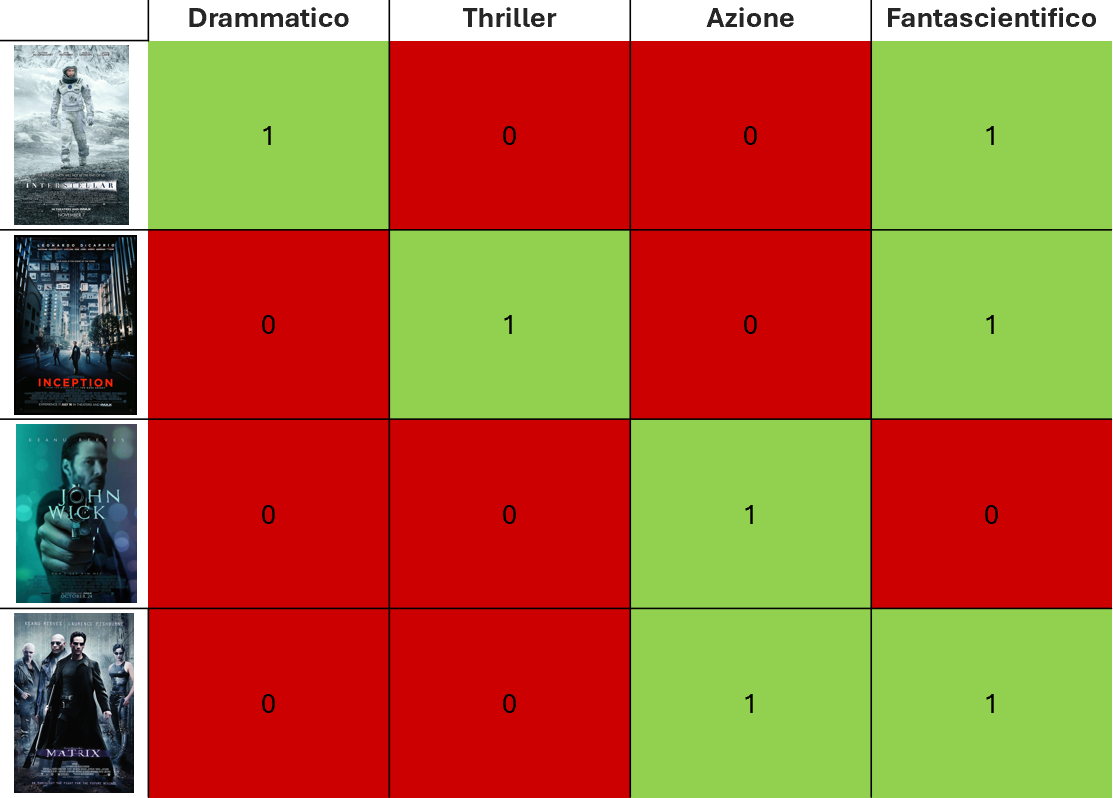
\includegraphics[scale=0.5]{figures/content_based_filtering.PNG}
    \caption{La figura mostra i vettori delle caratteristiche dei film (in questo caso il genere) per i film in esempio. Se il film appartiene ad uno specifico genere viene posto il valore $1$, altrimenti $0$}
    \label{fig:item_vector}
\end{figure}

Si creano vettori per i film considerando tutti i generi analizzati fino ad ora e si calcola la similarità con il profilo dell'utente. Si ottiene, utilizzando per esempio la similarità coseno, un valore di $0.47$ per $Interstellar$ e di $0.67$ per \textit{John Wick}, quindi quest'ultimo viene raccomandato prima di \textit{Interstellar}, perché è più simile al profilo dell'utente.


\subsubsection{Vantaggi e svantaggi}

I vantaggi di quest'approccio sono:
\begin{itemize}
    \item il modello non ha bisogno di dati su altri utenti, poiché le raccomandazioni sono specifiche per questo utente. Questo lo rende più facile da scalare a un grande numero di utenti
    \item il modello può catturare gli interessi specifici di un utente e può raccomandare \textit{item} di nicchia che interessano a pochissimi altri utenti
\end{itemize}

Gli svantaggi di quest'approccio sono:
\begin{itemize}
    \item poiché la rappresentazione delle caratteristiche degli oggetti è in parte progettata manualmente, questa tecnica richiede molta conoscenza del dominio. Il modello può essere solo quindi valido quanto le caratteristiche progettate manualmente
    \item il modello può fare raccomandazioni solo basate sugli interessi esistenti dell'utente. In altre parole, ha una capacità limitata di espandere gli interessi dell'utente
\end{itemize}

\section{Collaborative filtering}
Il \textit{collaborative filtering} (\textit{CF}) viene introdotto per la prima volta dal sistema \textit{Tapestry}~\cite{Tapestry} e si riferiva al fatto che ``people collaborate to help one another perform the filtering process in order to handle the large amounts of email and messages posted to newsgroups". Questo termine ha poi assunto significati più ampi. In senso generale, indica il processo di filtraggio di informazioni o pattern tramite tecniche che coinvolgono la collaborazione tra più utenti, agenti e fonti di dati. Il \textit{CF} esiste in molte forme e, sin dalla sua introduzione, sono stati proposti numerosi metodi basati su di esso.

Per affrontare alcune delle limitazioni del \textit{content-base filtering}, il \textit{collaborative filtering} utilizza simultaneamente le somiglianze tra utenti e \textit{item} per fornire raccomandazioni. I modelli possono raccomandare un \textit{item} all'utente $A$ in base agli interessi di un utente simile $B$ anche se $A$ non ha mai visto \textit{item} simili. Inoltre, gli \textit{embedding}, se presenti, possono essere appresi automaticamente senza dover progettare manualmente le caratteristiche.

In generale, le tecniche di \textit{CF} possono essere suddivise in tre categorie: \textit{CF} basato sulla memoria, \textit{CF} basato su modelli e i modelli ibridi~\cite{Su}. Tra le tecniche rappresentative basate sulla memoria ci sono i metodi \textit{nearest neighbor-based}~\ref{knn}, come il \textit{CF} basato sugli utenti (\textit{user-based}) e quello basato sugli oggetti (\textit{item-based})~\cite{Sarwar}. I modelli a fattori latenti, come la \textit{Matrix Factorization}~\ref{matrix_factorization}, sono esempi di \textit{CF} basato su modelli. Il \textit{CF} basato sulla memoria presenta delle limitazioni nella gestione di dati sparsi e su larga scala, poiché calcola la similarità basandosi sugli oggetti in comune. I metodi basati su modelli sono diventati più popolari grazie alla loro maggiore efficacia nel gestire la sparsità e la scalabilità. Molti approcci \textit{CF} basati su modelli possono essere estesi con reti neurali, permettendo modelli più flessibili e scalabili grazie all’accelerazione computazionale offerta dal \textit{Deep Learning}~\cite{Zhang}. In generale, il \textit{CF} utilizza solo i dati di interazione tra utenti e oggetti per fare previsioni e raccomandazioni. Oltre al \textit{CF}, anche i sistemi di raccomandazione \textit{content-based} e \textit{context-based} sono utili per includere descrizioni dei contenuti degli oggetti/utenti e segnali contestuali come timestamp e localizzazione. Ovviamente, è necessario adattare i tipi o le strutture dei modelli in base ai dati in input disponibili.

Si consideri un sistema di raccomandazione di film in cui i dati di addestramento consistono in una matrice di feedback in cui:

\begin{itemize}
    \item Ogni riga rappresenta un utente
    \item Ogni colonna rappresenta un \textit{item} (un film)
    \item Il feedback sui film rientra in una delle due categorie:
    \begin{itemize}
        \item esplicito: gli utenti specificano quanto gli è piaciuto un determinato film fornendo una valutazione numerica
        \item implicito: se un utente guarda un film, il sistema deduce che l'utente è interessato
    \end{itemize}
\end{itemize}

Per semplificare, si supponga che la matrice di feedback sia binaria; cioè, un valore di $1$ indica interesse per il film.

Quando un utente visita la homepage, il sistema dovrebbe raccomandare film basati su:

\begin{enumerate}
    \item somiglianza con i film che l'utente ha apprezzato in passato
    \item film che utenti simili hanno apprezzato
\end{enumerate}

\subsection{1D embedding}

Si assegna a ciascun film uno scalare in $[-1, 1]$ che descriva se il film è destinato a bambini (valori negativi) o ad adulti (valori positivi). Allo stesso modo, per ciascun utente si assegna uno scalare in $[-1, 1]$ che descriva il suo interesse per i film per bambini o per adulti. Il prodotto dell'\textit{embedding} del film e dell'\textit{embedding} dell'utente dovrebbe essere più alto (vicino a 1) per i film che dovrebbero piacere all'utente.

\begin{figure}[H]
    \centering
    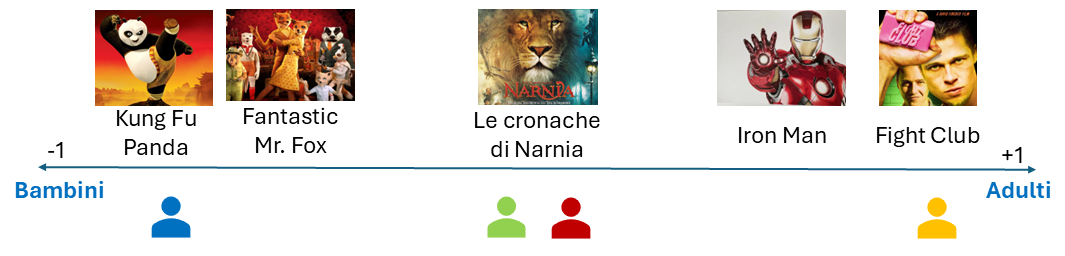
\includegraphics[scale=0.4]{figures/collaborative_filtering/embeddings.PNG}
    \caption{Rappresentazione su un asse 1D delle posizioni di utenti e film rispetto allo scalare assegnato nell'intervallo $[-1, 1]$}
    \label{fig:embeddings}
\end{figure}

Nella seguente matrice, ogni segno di spunta identifica un film che un determinato utente ha guardato. Il terzo e il quarto utente hanno preferenze evidenti per questa caratteristica: il terzo utente preferisce i film per bambini, mentre il quarto preferisce i film per adulti. Ciò non vale invece per il primo e del secondo utente.

\begin{figure}[H]
    \centering
    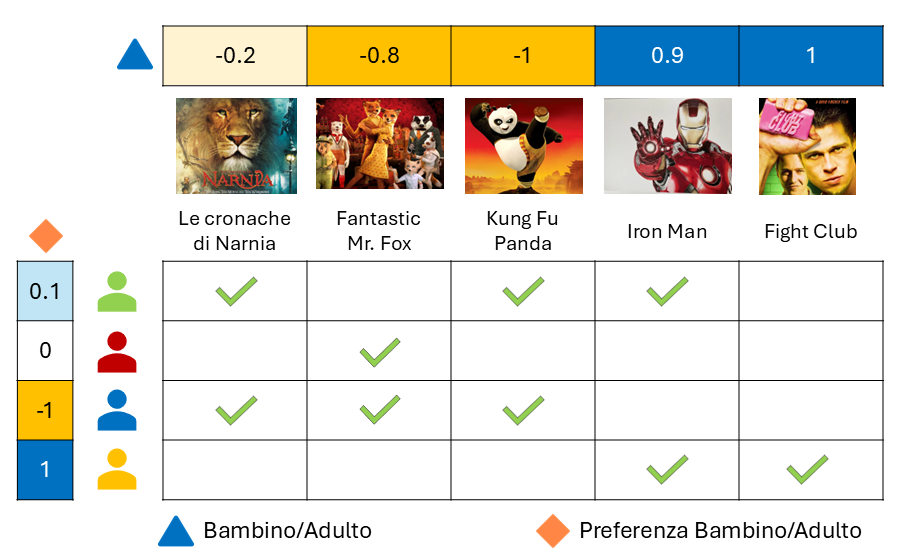
\includegraphics[scale=0.5]{figures/collaborative_filtering/1D_matrix.PNG}
    \caption{matrice che mostra i film guardati dagli utenti, le categorie dei film e le preferenze degli utenti}
    \label{fig:1D_matrix}
\end{figure}

\subsubsection{2D embedding}

Una sola caratteristica non è sufficiente a spiegare le preferenze di tutti gli utenti. Per superare questo problema, si utilizza una seconda caratteristica: il grado in cui ogni film è un \textit{blockbuster} (film molto popolare e di grande successo al botteghino) o un film d'autore. Con una seconda caratteristica, ora si può rappresentare ogni film con il seguente \textit{embedding} bidimensionale:

\begin{figure}[H]
    \centering
    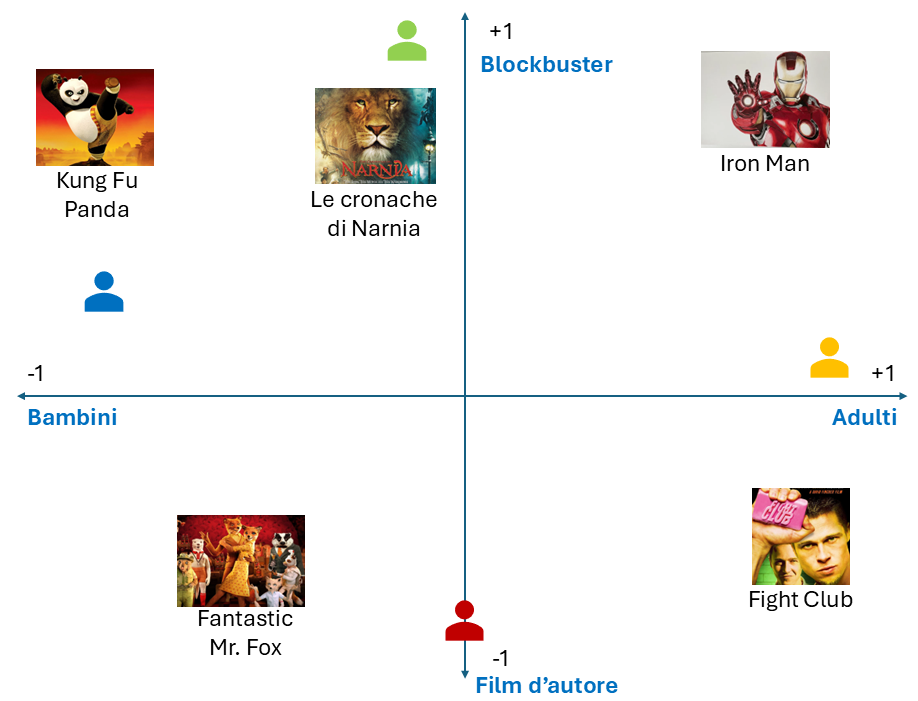
\includegraphics[scale=0.4]{figures/collaborative_filtering/axes.PNG}
    \caption{gli assi mostrano, per ciascuna caratteristica, la posizione dei film e le preferenze degli utenti}
    \label{fig:embedding_axes}
\end{figure}

Nel grafico sono rappresentati sia gli elementi che gli utenti nello stesso spazio di \textit{embedding}. Questo perché si può pensare allo spazio di \textit{embedding} come a una rappresentazione astratta comune sia agli \textit{item} che agli utenti, in cui si può misurare la similarità.

\begin{figure}[H]
    \centering
    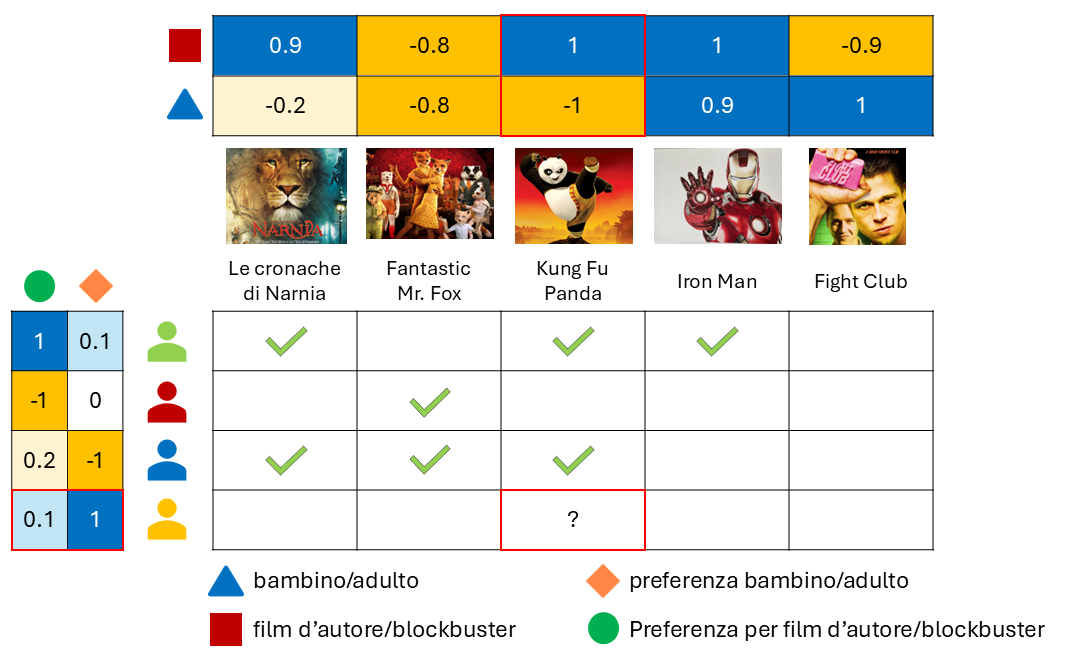
\includegraphics[scale=0.4]{figures/collaborative_filtering/2D_matrix.PNG}
    \caption{matrice che mostra i film guardati dagli utenti, le categorie dei film e le preferenze degli utenti estese}
    \label{fig:2D_matrix}
\end{figure}

L'obbiettivo è che per ogni coppia (utente, \textit{item}) il prodotto scalare dell'\textit{embedding} dell'utente e dell'\textit{embedding} dell'\textit{item} fosse vicino a $1$ quando l'utente ha guardato il film e a $0$ in caso contrario.

I modelli apprendono automaticamente un vettore di \textit{embedding} per ciascun utente che spieghi al meglio le sue preferenze. Di conseguenza, gli \textit{embedding} di utenti con gusti simili risulteranno vicini tra loro. Allo stesso modo il modello apprende gli \textit{embedding} dei film in modo da spiegare al meglio la matrice di feedback. Anche in questo caso, gli \textit{embedding} dei film apprezzati da utenti simili saranno vicini nello spazio degli embedding.

\subsubsection{Vantaggi e svantaggi}

I vantaggi di quest'approccio sono:

\begin{itemize}
  \item non è necessaria conoscenza del dominio: gli embedding vengono appresi automaticamente
  \item serendipità: anche se il modello non sa che l'utente è interessato a un determinato \textit{item} potrebbe comunque raccomandarlo perché utenti simili sono interessati a quell'\textit{item}
  \item ottimo punto di partenza: il sistema ha bisogno solo della matrice di feedback, e non di informazioni contestuali, per addestrare un modello
\end{itemize}

Gli svantaggi di quest'approccio sono:

\begin{itemize}
  \item non si può gestire \textit{item} nuovi: se un oggetto non è stato visto durante l'addestramento, il sistema non può creare un \textit{embedding} per esso. Questo problema è noto come \textit{cold-start}. Tuttavia, esistono tecniche che possono affrontare in parte questo problema: 

  \begin{itemize}
    \item proiezione: dato un nuovo \textit{item} $i_0$ non visto durante l'addestramento, se il sistema ha alcune interazioni con utenti, può facilmente calcolare un \textit{embedding} per quell'\textit{item} senza riaddestrare l'intero modello. Basta risolvere la seguente equazione (o la sua versione pesata):

    \[
    \min_x \sum_{i}(r_{ui} - x^T u_i)^2
    \]

    Gli \textit{embedding} dell'utente vengono mantenuti fissi, e il sistema risolve per ottenere l'\textit{embedding} dell'\textit{item}. Lo stesso approccio può essere utilizzato per un nuovo utente
    \item euristiche: se il sistema non ha interazioni, può approssimare l'\textit{embedding} di un \textit{item} facendo la media degli \textit{embedding} di \textit{item} appartenenti alla stessa categoria
  \end{itemize}

  \item difficoltà nell'includere caratteristiche aggiuntive per \textit{query}/\textit{item}: le caratteristiche aggiuntive (\textit{side features}) sono tutte quelle informazioni oltre all'ID della query o dell'\text{item}. Per esempio, per i film, le caratteristiche possono includere il paese o l'età. Includere queste caratteristiche migliora la qualità del modello

  Per generalizzare alcuni algoritmi, ad esempio \textit{WALS}~\ref{als} (\textit{Weighted Alternating Least Squares}, metodo di \textit{Matrix Factorization}~\ref{matrix_factorization}), si può estendere la matrice di input includendo le caratteristiche, definendo una matrice a blocchi $\tilde{R}$:

  \[
  \tilde{R} = \begin{bmatrix}
  R & U_f \\
  I_f & 0
  \end{bmatrix}
  \]

  dove:
  \begin{itemize}
    \item $R$ è la matrice di feedback tra utenti e \textit{item};
    \item $U_f$ è una codifica multi-hot delle feature degli utenti (per esempio età, paese, genere)
    \item $I_f$ è una codifica multi-hot delle feature degli \textit{item} (per esempio categoria, lingua, creatore)
    \item $0$ è una matrice di zeri, che rappresenta l'assenza di interazioni dirette tra le feature utente e quelle degli \textit{item}
  \end{itemize}
\end{itemize}

\subsubsection{Approcci}


Esistono due approcci principali per facilitare tale confronto, che costituiscono le due tecniche fondamentali del \textit{collaborative filtering}: 

\begin{itemize}
    \item approcci \textit{neighborhood}: si concentrano sulle relazioni tra \textit{item} oppure, alternativamente, tra utenti. Un approccio \textit{item}-\textit{item} modella la preferenza di un utente per un \textit{item} sulla base delle valutazioni di \textit{item} simili da parte dello stesso utente
    \item modelli basati sulla \textit{Matrix Factorization}: un approccio in cui sia gli \textit{item} che gli utenti vengono proiettati in uno stesso spazio latente, cercando di spiegare le valutazioni osservate attraverso fattori latenti inferiti automaticamente dai feedback
\end{itemize}

\section{Matrix Factorization}\label{matrix_factorization}

La \textit{Matrix Factorization} è una tecnica utilizzata per rappresentare una matrice come prodotto di due o più matrici. Consente di estrarre strutture latenti dai dati, rendendo possibile la scoperta di relazioni implicite tra entità \cite{MC}.

Questa tecnica è alla base di molte applicazioni in ambiti diversi, tra cui l'elaborazione di segnali, la compressione dei dati, la visione artificiale e, in particolare, i sistemi di \textit{recommendation}.

Formalmente, data una matrice $R \in \mathbb{R}^{m \times n}$, la fattorizzazione mira a trovare due matrici $W \in \mathbb{R}^{m \times k}$ e $H \in \mathbb{R}^{n \times k}$ tali che:
\[
R \approx WH^T
\]
dove 
\begin{itemize}
    \item le righe di $W$ corrispondono agli \textit{embedding} degli utenti
    \item le righe di $H$ corrispondono agli \textit{embedding} degli \textit{item}
    \item $k \ll \min(m,n)$ è il rango latente scelto
\end{itemize}

\begin{figure}[H]
    \centering
    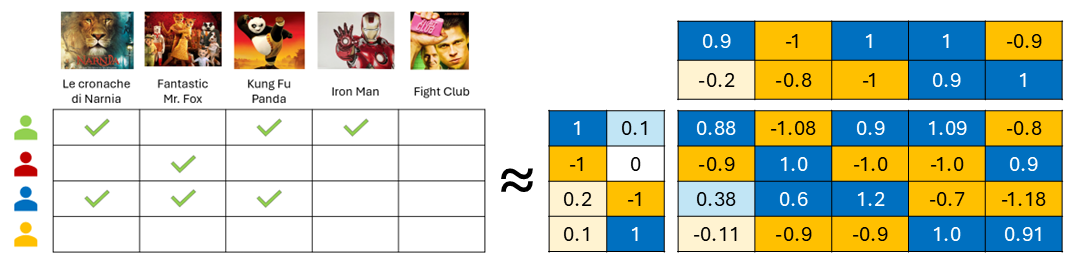
\includegraphics[scale=0.5]{figures/matrix_factorization.PNG}
    \caption{rappresentazione della matrice $R$ come prodotto delle due matrici $W$ e $H$}
    \label{fig:matrix_factorization}
\end{figure}

Questa approssimazione riduce la dimensionalità dei dati, semplifica il modello e cattura le relazioni principali presenti nella matrice originaria.

Un celebre esempio dell'efficacia di questa tecnica nei sistemi di \textit{recommendation} è il \textit{Netflix Prize} del 2006. Il team vincente la utilizzò per migliorare le previsioni di rating del 10\% rispetto al sistema originario di Netflix \cite{TheNP}.

I principali vantaggi nel suo utilizzo sono la scalabilità, poiché i modelli sono efficienti da memorizzare e computare, e la capacità di generalizzazione, in quanto riescono a catturare relazioni latenti non esplicitamente osservate. Tuttavia, esistono anche alcuni limiti, tra cui il problema della \textit{cold start}, che rende difficile raccomandare per nuovi utenti o nuovi \textit{item}, e la sparsità, che può portare a una una bassa qualità delle raccomandazioni\cite{SVD_analysis}.

Pur con alcune limitazioni, essa costituisce la base per molti degli algoritmi di \textit{recommendation} più efficaci oggi in uso, ed è spesso integrata con approcci più complessi, come i modelli Deep Learning o i grafi.

\section{Tipologie di feedback}

I sistemi di raccomandazione si basano sull'analisi delle preferenze degli utenti, espresse attraverso due principali modalità: feedback esplicito e feedback implicito~\cite{ALS}. Ogni modalità presenta vantaggi, limitazioni e diverse tipologie di approcci. 

Poiché ciascuna forma di feedback fornisce informazioni diverse, un approccio ibrido è spesso preferibile. Ad esempio, nei sistemi che dispongono di valutazioni esplicite, il feedback implicito può essere utilizzato per arricchire il contesto dell'utente, migliorando le prestazioni del modello nei casi in cui i dati espliciti siano scarsi. I modelli basati sul Deep Learning possono essere progettati per combinare diverse fonti, sfruttando il feedback implicito arricchito da attributi contestuali (tempo, luogo, dispositivo, ecc.) per ottimizzare la previsione.

\subsection{Feedback Esplicito}

Il feedback esplicito si riferisce a tutte quelle situazioni in cui l'utente comunica consapevolmente il proprio grado di interesse per un oggetto. Esempi includono le valutazioni da $1$ a $5$ stelle per i prodotti su \textit{Amazon} o il pollice su/giù per i video su \textit{YouTube} o semplicemente il \textit{like} su \textit{Instagram}.

I modelli che utilizzano feedback espliciti predicono il \textit{rating} che un dato utente assegnerebbe ad un \text{item}. Per esempio predicono che l'utente $u$ darebbe una votazione di $4$ su $5$ per la serie $i$.

Questi dati forniscono un segnale diretto, ma presentano però anche delle limitazioni:

\begin{itemize}
    \item più difficili da ottenere: richiedono che l'utente lasci intenzionalmente il suo riscontro
    \item rari nel mondo reale: molti utenti non lasciano mai valutazioni, dando origine a dati molto sparsi
    \item possono introdurre bias: ad esempio, utenti soddisfatti sono più propensi a lasciare valutazioni rispetto a quelli neutrali o insoddisfatti o viceversa
\end{itemize}

Nonostante ciò, il feedback esplicito rimane una delle fonti più affidabili per l'addestramento di modelli di raccomandazione, in quanto consente di formulare il problema come una regressione delle valutazioni mancanti~\cite{Implicit_feedback}.

\subsection{Feedback Implicito}

Il feedback implicito, al contrario, non è fornito direttamente dall'utente, ma viene dedotto osservando i suoi comportamenti. Esempi tipici includono:

\begin{itemize}
    \item cronologia degli acquisti
    \item cronologia di navigazione
    \item pattern di ricerca
    \item tempo di permanenza su una pagina
    \item interazioni come click, visualizzazioni o movimenti del mouse
    \item acquisto o meno di un prodotto
\end{itemize}

I feedback impliciti possono essere raccolti facilmente in modo automatico e passivo senza che l'utente debba interagire intenzionalmente. Inoltre, sono molto più abbondanti rispetto alla controparte esplicita. Forniscono una rappresentazione più completa del comportamento degli utenti, specialmente in contesti in cui il feedback esplicito è assente o insufficiente. Allo stato attuale, i modelli di \textit{Deep Learning} moderni utilizzano grandi quantità di feedback impliciti. 

I modelli che utilizzano feedback impliciti non forniscono un \textit{rating} ma uno \textit{score} numerico per la coppia utente-\textit{item}. Questo numero da solo non ha alcun significato, ma messo in relazioni con altri \textit{score}, calcolati per lo stesso utente con \textit{item} diversi, permette di ordinare gli \textit{item} in base alla preferenza predetta per l'utente.

L'utilizzo di dati impliciti può creare complicazioni:

\begin{itemize}
    \item ambiguità: un'azione (es. visualizzazione di un contenuto) non implica necessariamente una preferenza positiva
    \item rumore nei dati: molte interazioni potrebbero essere accidentali o non intenzionali
    \item assenza di segnali negativi chiari: è difficile distinguere tra mancanza di interesse e mancata esposizione all'oggetto
\end{itemize}
